%----------------------------------------------------------------------------------------
%	PACKAGES AND OTHER DOCUMENT CONFIGURATIONS
%----------------------------------------------------------------------------------------

\documentclass[11pt]{article}
%\input{mydef.tex}
\usepackage{fancyhdr} % Required for custom headers
\usepackage{lastpage} % Required to determine the last page for the footer
\usepackage{extramarks} % Required for headers and footers
\usepackage[usenames,dvipsnames]{color} % Required for custom colors
\usepackage{graphicx} % Required to insert images
\usepackage{listings} % Required for insertion of code
\usepackage{courier} % Required for the courier font
\usepackage{amssymb,amsmath}
\usepackage{amsfonts}
\usepackage{mathtools}
\usepackage{subfigure}
\usepackage{enumitem}
\usepackage{bm}
\usepackage{url}
\usepackage[stable]{footmisc}
\usepackage{booktabs}
\usepackage[square]{natbib}
\usepackage{indentfirst}
%\usepackage[colorlinks, linkcolor=red, anchorcolor=purple, citecolor=blue]{hyperref}
\usepackage{hyperref}
\usepackage{algorithm}
\usepackage{algpseudocode}

\usepackage{multicol}
\setlength{\columnsep}{1cm}

% Margins
\topmargin=-0.45in
\evensidemargin=0in
\oddsidemargin=0in
\textwidth=6.5in
\textheight=9.0in
\headsep=0.25in
\setlength{\headheight}{13.6pt}
\linespread{1.1} % Line spacing

% Set up the header and footer
\pagestyle{fancy}
\lhead{CS 57800} % Top left header
\chead{}
\rhead{Homework 3} % Top right header
\lfoot{} % Bottom left footer
\cfoot{} % Bottom center footer
\rfoot{Page\ \thepage\ of\ \protect\pageref{LastPage}} % Bottom right footer
\renewcommand\headrulewidth{0.4pt} % Size of the header rule
\renewcommand\footrulewidth{0.4pt} % Size of the footer rule

\renewcommand*{\thefootnote}{\fnsymbol{footnote}}

\setlength{\parskip}{.2\baselineskip}
%\setlength\parindent{0pt} % Removes all indentation from paragraphs

\title{
\textbf{CS57800 Statistical Machine Learning} \\ \textsc{Homework 3} \\
\normalsize\vspace{0.1in}
}

\author{
	\textbf{Ting Zhang} \\
	School of Industiral Engineering\\
	\texttt{zhan1013@purdue.edu}
}

\date{\today}
%----------------------------------------------------------------------------------------

\begin{document}

\maketitle
%\thispagestyle{empty}

\section{Foundations}
\begin{itemize}
\item[1.]
The VC dimension of C is \(2n+1\). For a convex polygon with \(n\) vertices, the VC dimension of it is \(2n+1\). Then, it is clear that for any polygon with \(n\) vertices, the VC dimension is at least \(2n+1\). Also, it can be shown that for \(2n+2\) points, there is always one point that can not be labeled correctly.
\item[2.] To show it is a convex function, we can compute the second derivative of the function.
\begin{align*}
& \frac{dl}{d\hat{y}} = \frac{1}{\log 2}[\frac{-ye^{-y\hat{y}}}{(1+e^{-y\hat{y}}) \log 2}] = \frac{1}{(\log 2)^2} (-1 + \frac{y}{1+e^{-y\hat{y}}})  \\
& \frac{d^2l}{d\hat{y}^2} =  \frac{1}{(\log 2)^2}[0 + y*(-2)*(\frac{1}{1+e^{-y\hat{y}}})^2 * (-y) * e^{-y\hat{y}}] = \frac{2y^2e^{-y\hat{y}}}{(\log 2)^2 (1+e^{-y\hat{y})}} > 0
\end{align*}
Since the second derivative of this function is greater than 0, then this function is a convex function.
\item[3.] The training error of the final hypothesis can be formulated as
\begin{equation*}
TrainingError(H_{final}) \leq \prod_{t} [2 \sqrt{\epsilon_t(1-\epsilon_t)}] \leq e^{-2 \sum_{t} (\gamma)^2}.
\end{equation*}
Since we want final hypothesis has training error of 0, then \(e^{-2 \sum_{t} (\gamma)^2} < 1/n\). This equation can be reformulated as \(-2T (1-\gamma)^2<-\ln n\). Therefore, we have \(T>\frac{\ln n}{2(1-\gamma)^2}\).
\item[4.] The decision boundary of each weak hypothesis is a axis-parallel line, as shown in Figure~\ref{fig:hw3_q4}. Positive points are represented with "+", and negative points are represented with "*". Then the process of doing Adaboost is as following: \\
\begin{figure}[!ht]
  \centering 
  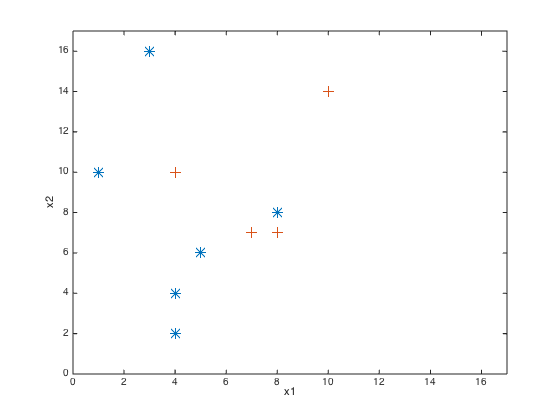
\includegraphics[width=0.5\columnwidth]{hw3_q4.png}%
  \caption{Examples shown in 2d representation.}
  \label{fig:hw3_q4}
\end{figure}
(1) First iteration \(t=1\), find the decision boundary that makes the least number of mistakes. In first iteration, each example is uniformlly distributed, with \(D_1(i)=0.1\). Here it found \(x_1>6\) and \( x_2>6\), with 3 mistakes, including example 1, 5 and 10. Therefore, the error is \(\epsilon_1=0.3\). The weak hypothesis is \(h_1(x_i): sign(x_1-6)*sign(x_2-6)\).\\
(2) Second iteration \(t=2\), first, update the distribution of each example. To update the distribution, we need to follow these euqations:
\begin{equation*}
\alpha_1 = 0.5 * \ln (\frac{1-\epsilon_1}{\epsilon_1}) = 0.5 * \ln (\frac{1-0.3}{0.3}) = 0.424
e_{-\alpha_1} = 0.654 
e_{\alpha_1} = 1.53
\end{equation*}
So, the distribution of the correctly classified examples \(i=2,3,4,6,7,8,9\) becomes
\begin{equation*}
D_2(i) = \frac{D_1(i) *e_{-\alpha_1} }{Z_1} = \frac{0.0654}{Z_1}
\end{equation*}
and the distribution of the wrongly classified examples \(i=1,5,10\) becomes
\begin{equation*}
D_2(i) = \frac{D_1(i) *e_{\alpha_1} }{Z_1} = \frac{0.153}{Z_1}
\end{equation*}
Since \(\sum_{i=1}^{10} D_2(i) = 1\), we have \((7*0.0654+3*0.153)/Z_1=1\). So, \(Z_1 = 0.9162\). Therefore, the distribution of the examples now become
\begin{equation*}
D_2(i) =
  \begin{cases}
    0.0714       & \quad \text{if } i=2,3,4,6,7,8,9\\
    0.1668           & \quad \text{if } i=1,5,10\\
  \end{cases}
\end{equation*}
Then, finding the weak hypothesis that has the smallest error \(\sum_{i=1} D_2(i)\), where \(i\) is the index of wrongly classified example. Then, it find the weak hypothesis to be \(h_2(x_i): sign(x_1-16)*sign(x_2-16)\), with four mistakes, including example 3, 6, 7, 9. And the error is \(\epsilon_2 = 0.2856\). We can also compute \(\alpha_2 = 0.5 * \ln (\frac{1-\epsilon_2}{\epsilon_2}) = 0.458 \). \\
Then, the final hypothesis is 
\begin{align*}
H_{final}(x) &= sign(\sum_{t} \alpha_t h_t(x)) \\
&= sign(0.0.424*sign(x_1-6)*sign(x_2-6) + 0.458*sign(x_1-16)*sign(x_2-16))
\end{align*}
\item[5.] To verify a kernel function, we need to proof the positive semi-definite property of it.
\begin{align*}
& \iint f(\vec{x})K(\vec{x},\vec{y})f(\vec{y})d\vec{x}d\vec{y} \\
& =\iint f(\vec{x})[\alpha K_1(\vec{x},\vec{y})+\beta K_2(\vec{x},\vec{y})]f(\vec{y})d\vec{x}d\vec{y} \\
& = \iint \alpha f(\vec{x})K_1(\vec{x},\vec{y})f(\vec{y})d\vec{x}d\vec{y} + \beta f(\vec{x})K_2(\vec{x},\vec{y})f(\vec{y})d\vec{x}d\vec{y} \\
& > 0*0 + 0*0 \\
& = 0
\end{align*}
Because, \(K_1(\vec{x},\vec{y})\) and \(K_2(\vec{x},\vec{y})\) are positive semi-definite, \(\alpha\) and \(\beta\) are all positive.
\item[6.] \(\xi\) is defined as the margin of the soft SVM. When an example is classified correctly, \(0 \leq \xi \leq 1\); while if an example is classified wrongly, then \(\xi > 1\). Therefore, with \(M\) examples, there are at most \(M\) mistakes. Since  \(\xi > 1\), then \(\sum_{i=1}^{M} \xi_i > M*1 = M\). Therefore, \(\sum_{i=1}^{M} \xi_i\) is the upper bound on the training error of the classifier.
\end{itemize}

%x2>8: 0.25
%10:0.38
%8:0.476

\section{Programming Report}
In this assignment, Gradient decent algorithm with hinge lost is implemented. Two forms of regularization term are applied, including the "l1" and "l2" norm of weights. As the last homework, three features are experimented in this task, including the unigram, bigram and both unigram and bigram feature set. Four performance of these features and different regularization terms are measured, including the accuracy, precision, recall and f-score. Detail explanation is presented below.
\subsection{Gradient Decent}
In this gradient decent algorithm, hinge lost is applied with two forms of regularization, "l1" and "l2" norm. Hinge lost can be computed using the following equation:
\begin{equation*}
loss(y,f(x)) = max(0, 1-yf(x))
\end{equation*}
where \(f(x) = wx+b\). And the general form of norm for the weight, \(w\), can be represented as:
\begin{equation*}
||w||_p = (\sum_{d} |w_d|^p)^{\frac{1}{p}}
\end{equation*}
Then, for "l1" norm, it would be \(||w|| = (\sum_{d} |w_d|)\). And for "l2" norm, it would be  \(||w||_2 = \sqrt{\sum_{d} |w_d|^2}\). \\
In the gradient decent algorithm, we are going to minimize the objective function, \(loss(y,f(x))+\lambda R(w)\), where \(R(w)\) is the regularization term. To compute the gradient of this objective function, we can get:
\begin{itemize}
\item[*] loss function
\begin{equation*}
g(w) =
  \begin{cases}
    0       & \quad \text{if } y(wx+b)>1\\
    yx           & \quad \text{otherwise}\\
  \end{cases}
\end{equation*}
\item[*] l1: \(g(w) = sign(w)\)
\item[*] l2: \(g(w) = w\)
\end{itemize}
Therefore, the algorithm can be written as in Algorithm 1.
\begin{algorithm}
\caption{Gradient Decent algorithm with hinge lost}
%\label{CHalgorithm}
\begin{algorithmic}[1]
\Procedure{Gradient Decent}{}
\State $w = (0,0,...,0), b = 0 $
\For{iter = 1:MaxIterations }
\State$ g=(0,0,...,0), gb=0$
\For{$(x,y) \in D$}
\If {$y(wx+b) \leq 1$}
\State $g = g + yx$
\State$gb = gb + y$
\EndIf
\EndFor
\If {regularization == "l1"}
\State $g=g-\lambda sign(w)$
\ElsIf {regularization == "l2"}
\State $g=g- \lambda w$
\EndIf
\State$w = w + \eta g$
\State$b = b + \eta gb$
\EndFor
\EndProcedure
\end{algorithmic}
\end{algorithm}
\subsection{Experiment}
Experiments are conducted by selecting the correct parameters and with different feature set and regularization terms.
\subsubsection{Parameters}
For the gradient decent algorithm, there are several parameters, including the stepSize, regularization coefficient, \(\lambda\), and the number of iterations. In this task, the number of iterations is used as a hyper-parameter that tuned with a validation set. The parameter stepSize is selected empirically, the value of objective function is checked when selecting this parameter. When the objective function start to increase with a relatively small number of iterations, the stepSize is considered as too large. Multiple values are experimented and 0.0001 is selected. The regularization coefficient is used to control the complexity of the trained model. It is selected as 1.
\subsubsection{Results}
Experiments are conducted with 1000 iterations as maximum. The preformance are shown below.
\begin{itemize}
\item[*] "l1": Figure \ref{fig:I1_accuracy} shows the accuracy of training and validation for each feature set with "l1" regularization, over 1000 iterations. The precision, recall and f-score for training and validation set for each feature set is shown in Figure \ref{fig:I1_unigram}, \ref{fig:I1_bigram}, and \ref{fig:I1_bogram}, respectively. From Figure \ref{fig:I1_accuracy}, the number of iterations for the test set is decided. For unigram feature set, after 600 iterations, the accuracy for validation set is not growing. To avoid overfitting, 600 iterations is selected for the test test. For bigram feature set, the validation accuracy starts decreasing around 400 iterations, therefore, 400 iterations is selected for bigram feature set. For the one using both feature set, the validation accuracy decreases around 300 iterations. Therefore, 300 is selected for it. The test performance for unigram, bigram and both feature set is shown in Table \ref{I1_test}.
\begin{figure}[!h]
  \centering 
	\subfigure[]{\label{fig:a}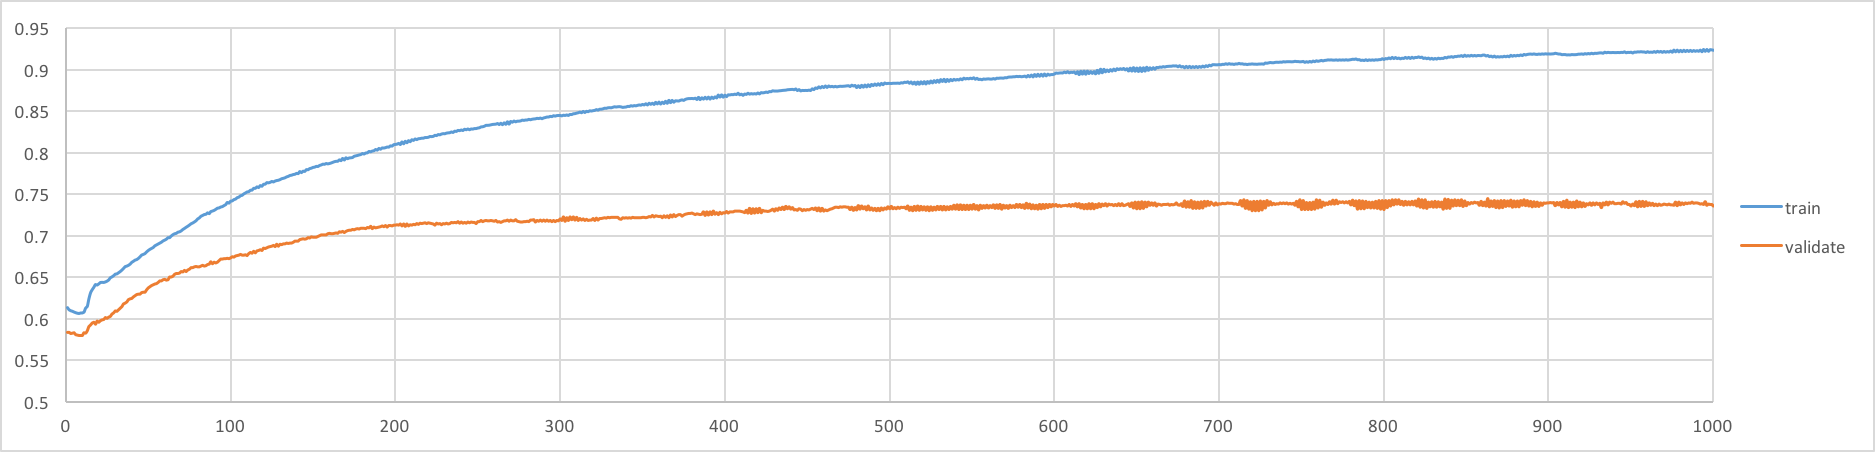
\includegraphics[width=1.0\columnwidth]{I1_uni.png}}\\%
	\subfigure[]{\label{fig:b}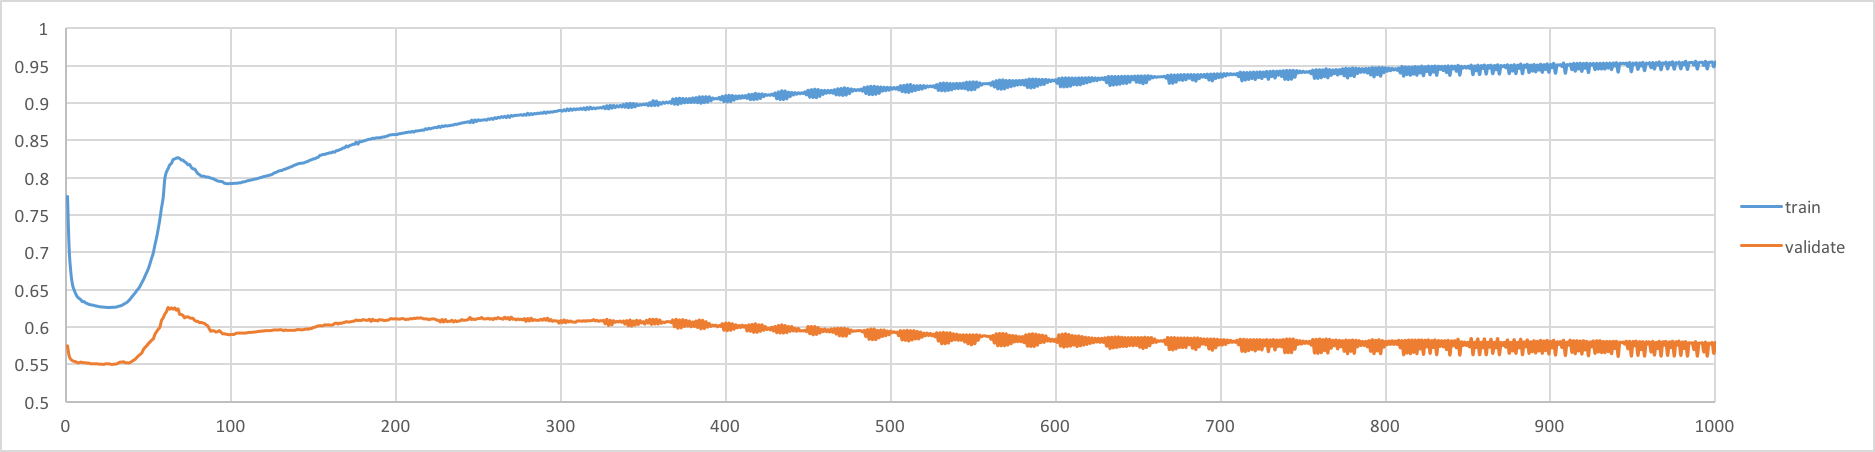
\includegraphics[width=1.0\columnwidth]{I1_bi.png}}\\ % 
	\subfigure[]{\label{fig:c} 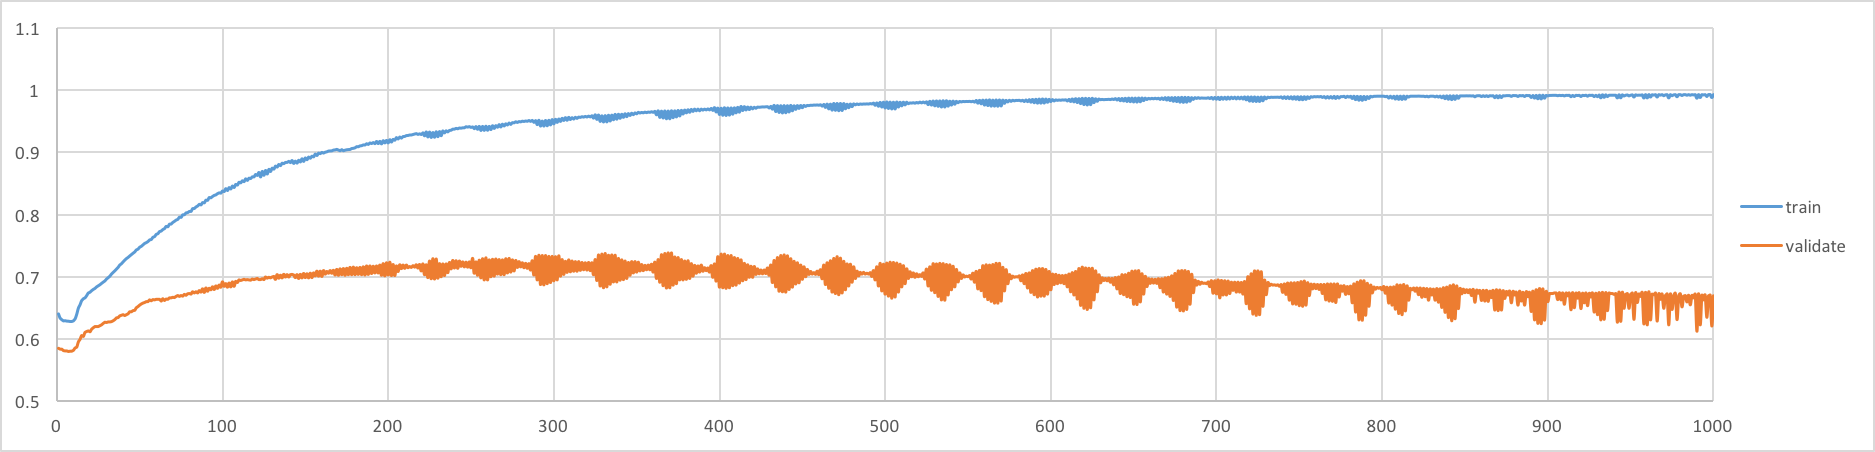
\includegraphics[width=1.0\columnwidth]{I1_both.png}}% 
%  \subfigure[Fibers bonded in the network.]{\label{fig:microstructure_mag} \includegraphics[width=0.5\columnwidth]{microstructure_mag.jpg}}% 
  \caption{Accuracy of training and validation set for different feature sets with I1 norm.}
  \label{fig:I1_accuracy}
\end{figure}

\begin{table}[]
\centering
\caption{Test performance of I1 norm for different feature set}
\label{I1_test}
\begin{tabular}{lllll}
\hline
        & Accuracy & Precision & Recall & F-score \\ \hline
Unigram & 0.75     & 0.76      & 0.72   & 0.74    \\ \hline
Bigram  & 0.61     & 0.82      & 0.28   & 0.42    \\ \hline
Both    & 0.75     & 0.78      & 0.67   & 0.72    \\ \hline
\end{tabular}
\end{table}

\item[*] "l2": Figure \ref{fig:I2_accuracy} shows the accuracy of training and validation for each feature set with "l2" regularization, over 1000 iterations. The precision, recall and f-score for training and validation set for each feature set is shown in Figure \ref{fig:I2_unigram}, \ref{fig:I2_bigram}, and \ref{fig:I2_bogram}, respectively. From Figure \ref{fig:I2_accuracy}, 600 iterations for unigram and bigram is selected for testing and 400 iterations is selected for the one using both feature set. The test performance for unigram, bigram and both feature set is shown in Table \ref{I2_test}.
\end{itemize}

\begin{table}[]
\centering
\caption{Test performance of I2 norm for different feature set}
\label{I2_test}
\begin{tabular}{lllll}
\hline
        & Accuracy & Precision & Recall & F-score \\ \hline
Unigram & 0.74     & 0.73      & 0.75   & 0.74    \\ \hline
Bigram  & 0.67     & 0.65      & 0.76   & 0.70    \\ \hline
Both    & 0.75     & 0.73      & 0.78   & 0.75    \\ \hline
\end{tabular}
\end{table}

\subsubsection{Comparisons}
For both "I1" and "I2" norm, unigram feature set and using both feature set shows relatively higher accuracy than bigram feature set. When comparing between "I1" and "I2" norm, it can be observed that "I2" norm shows less ocsillation. Another important observation is that, "I2" norm is less likely overfitting than "I1" norm. Comparing Figure \ref{fig:I1_accuracy} and Figure \ref{fig:I2_accuracy}, we can find "I1" norm validation accuracy decreases while the number of iterations increases. However, "I2" norm validation accuracy remains at a certain level while the number of iterations goes up.

\begin{figure}[!h]
  \centering 
	\subfigure[]{\label{fig:a}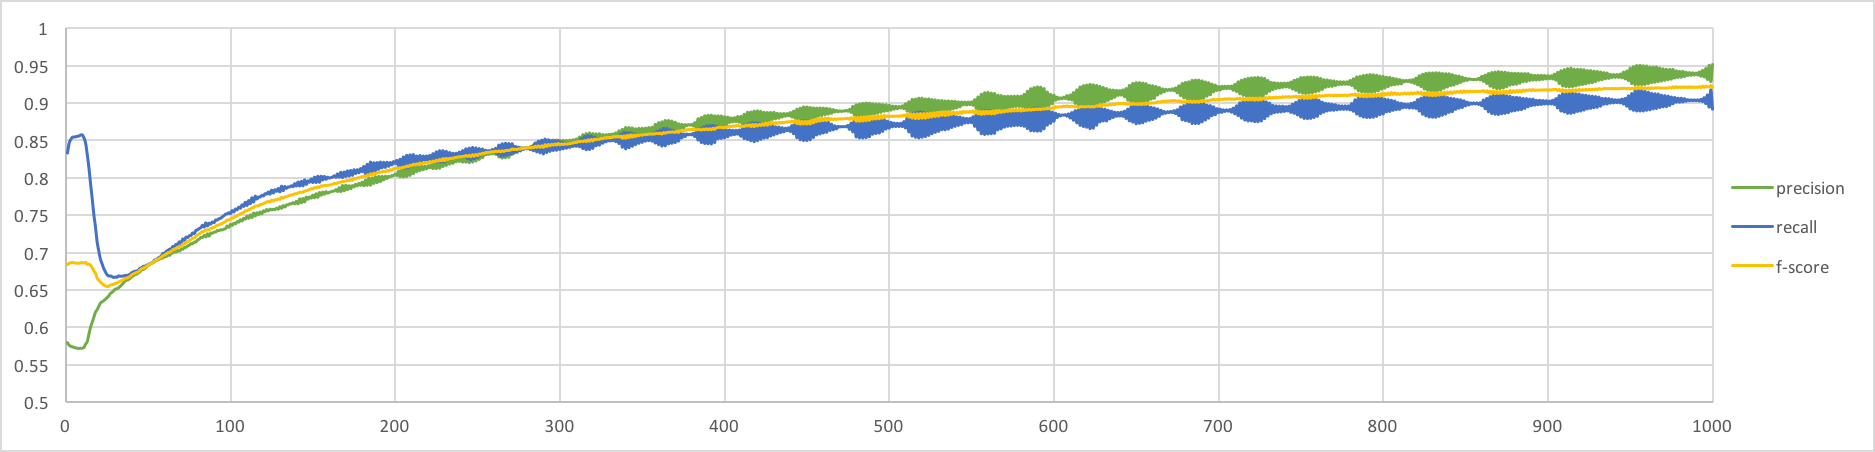
\includegraphics[width=1.0\columnwidth]{I1_uni_tr.png}}\\%
	\subfigure[]{\label{fig:b}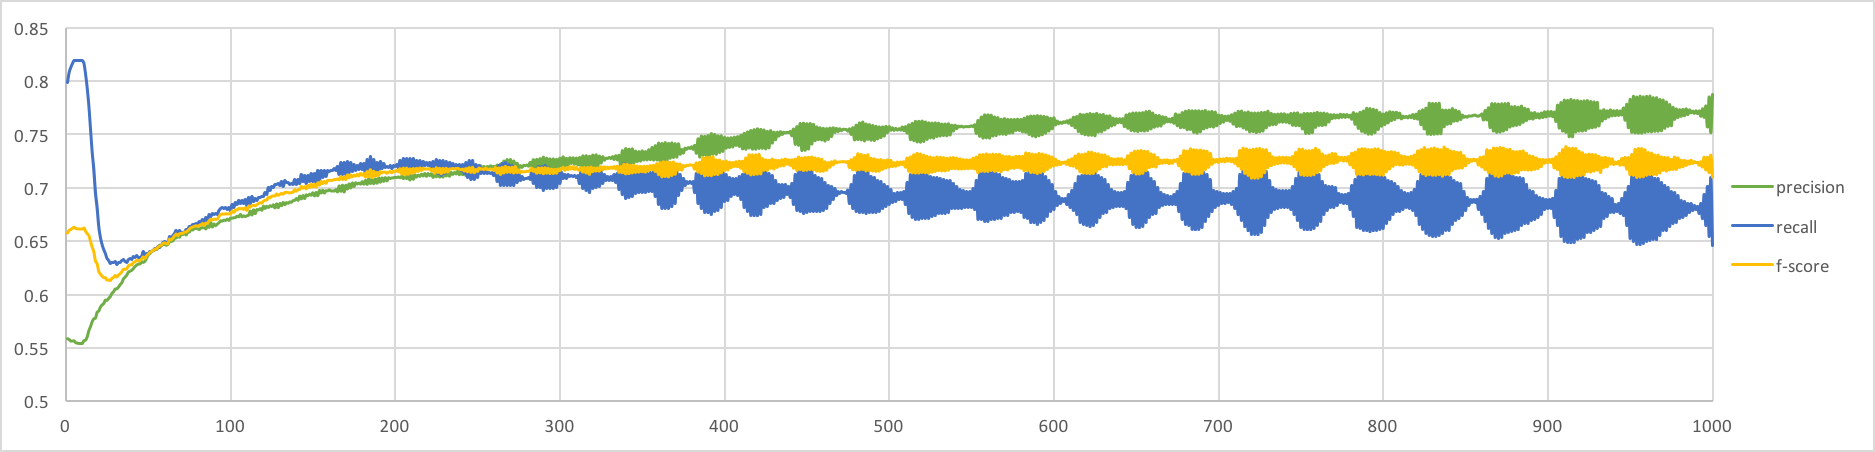
\includegraphics[width=1.0\columnwidth]{I1_uni_va.png}}%  
%  \subfigure[Fibers bonded in the network.]{\label{fig:microstructure_mag} \includegraphics[width=0.5\columnwidth]{microstructure_mag.jpg}}% 
  \caption{Performance of (a) training and (b) validation set for unigram feature sets with I1 norm.}
  \label{fig:I1_unigram}
\end{figure}

\begin{figure}[!h]
  \centering 
	\subfigure[]{\label{fig:a}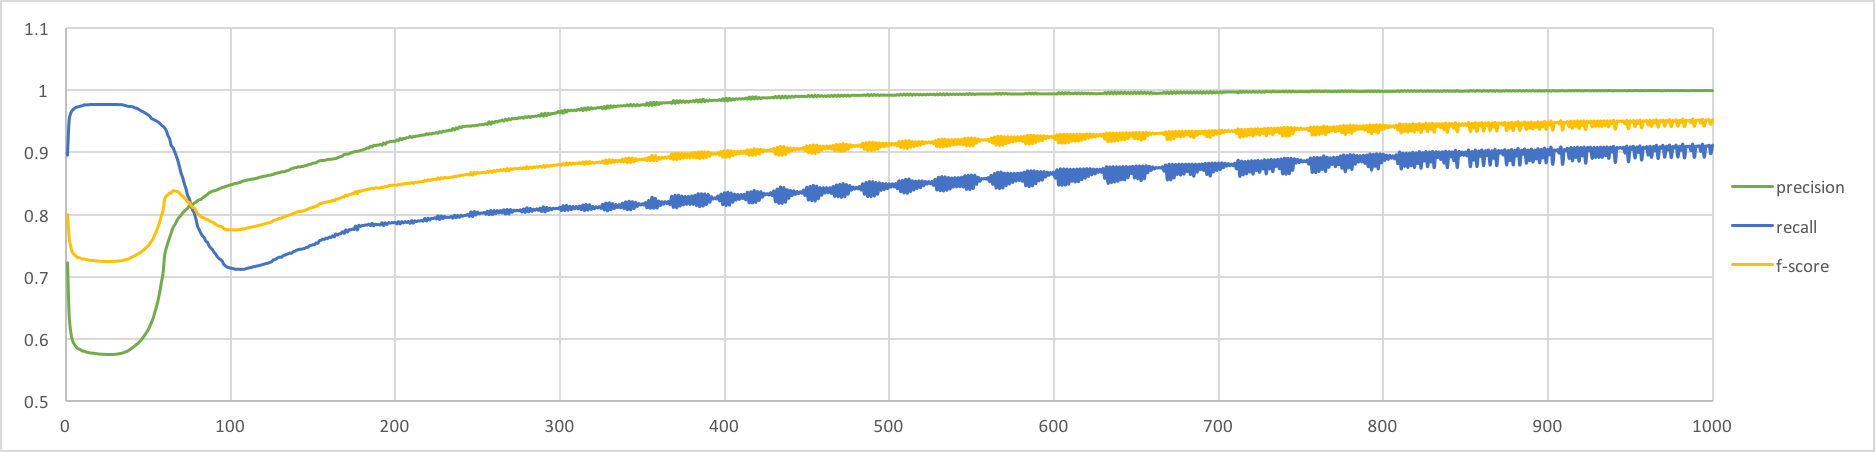
\includegraphics[width=1.0\columnwidth]{I1_bi_tr.png}}\\%
	\subfigure[]{\label{fig:b}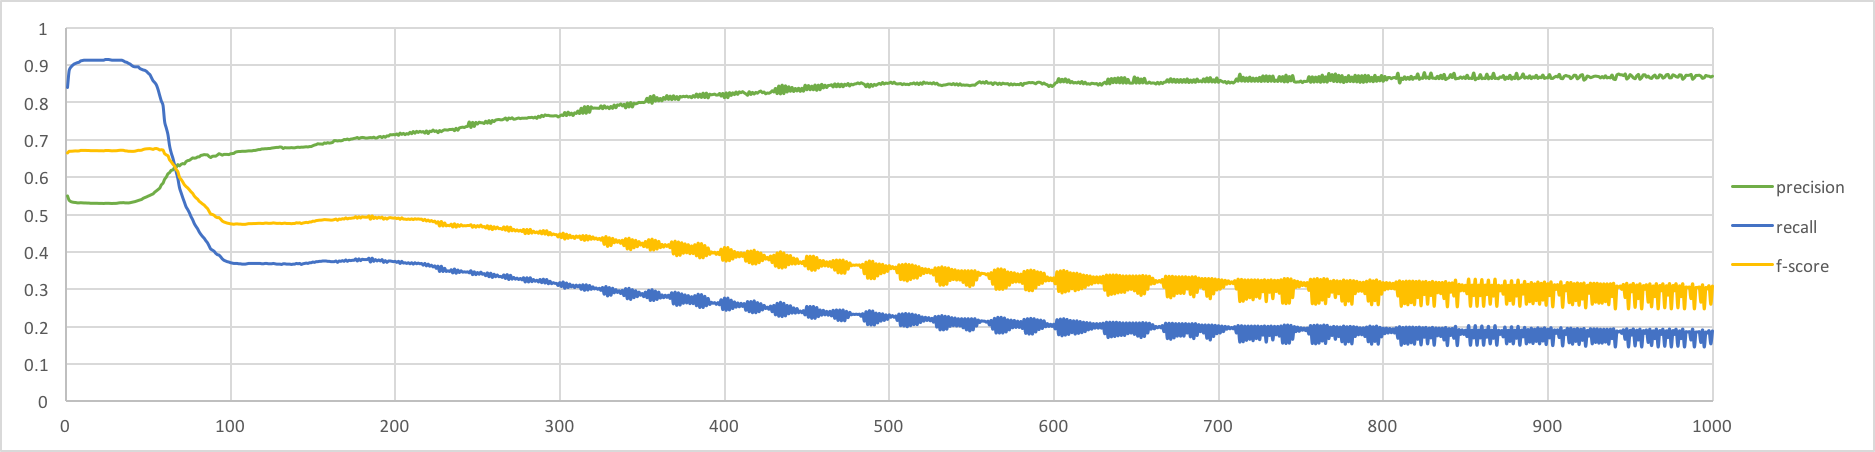
\includegraphics[width=1.0\columnwidth]{I1_bi_va.png}}%  
%  \subfigure[Fibers bonded in the network.]{\label{fig:microstructure_mag} \includegraphics[width=0.5\columnwidth]{microstructure_mag.jpg}}% 
  \caption{Performance of (a) training and (b) validation set for bigram feature sets with I1 norm.}
  \label{fig:I1_bigram}
\end{figure}

\begin{figure}[!h]
  \centering 
	\subfigure[]{\label{fig:a}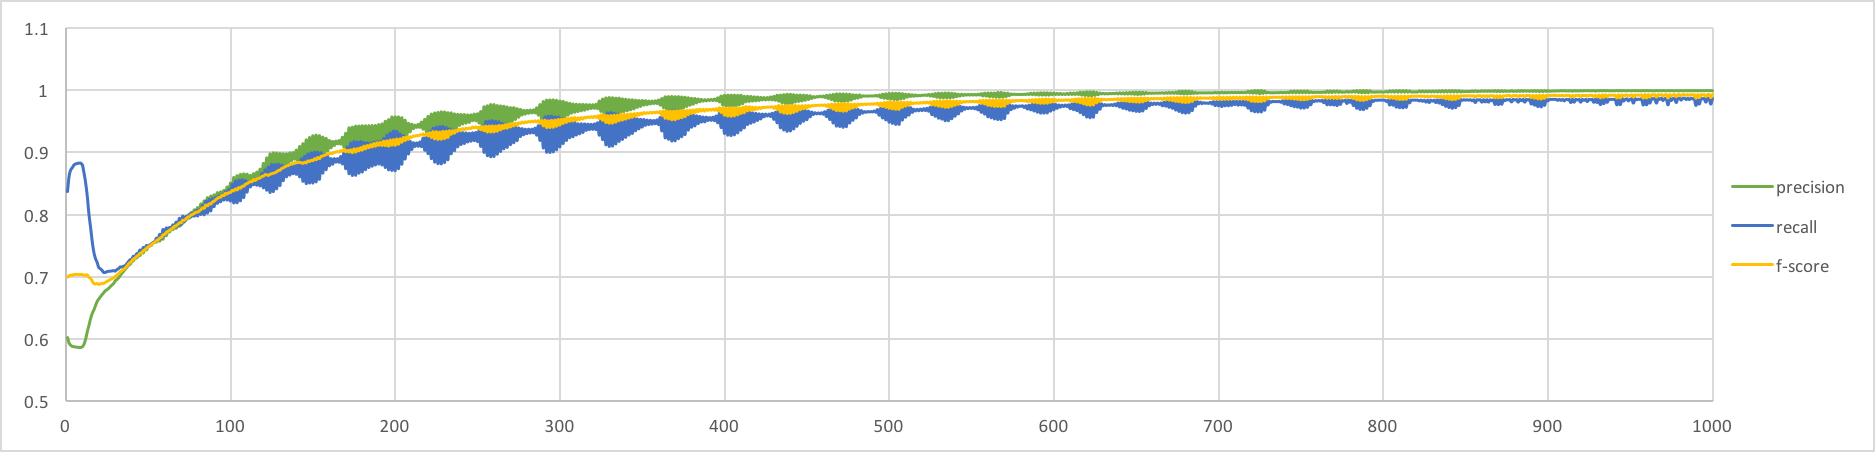
\includegraphics[width=1.0\columnwidth]{I1_bo_tr.png}}\\%
	\subfigure[]{\label{fig:b}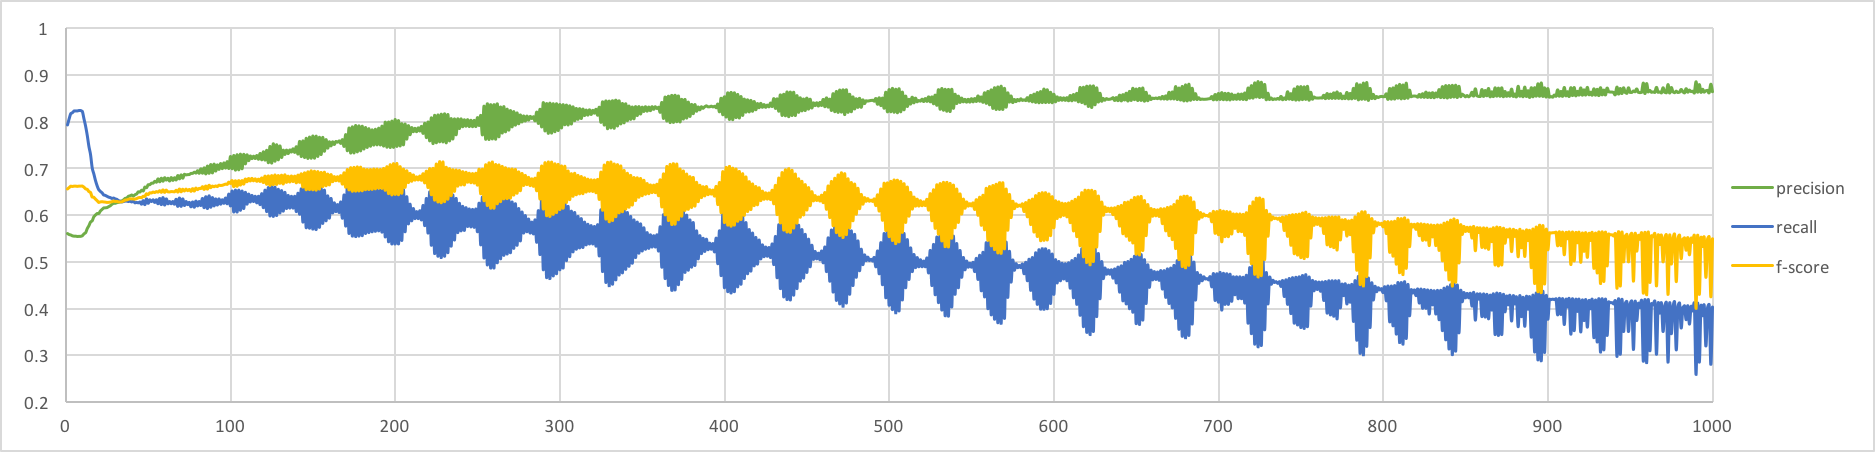
\includegraphics[width=1.0\columnwidth]{I1_bo_va.png}}%  
%  \subfigure[Fibers bonded in the network.]{\label{fig:microstructure_mag} \includegraphics[width=0.5\columnwidth]{microstructure_mag.jpg}}% 
  \caption{Performance of (a) training and (b) validation set for both feature sets with I1 norm.}
  \label{fig:I1_bogram}
\end{figure}

\begin{figure}[!h]
  \centering 
	\subfigure[]{\label{fig:a}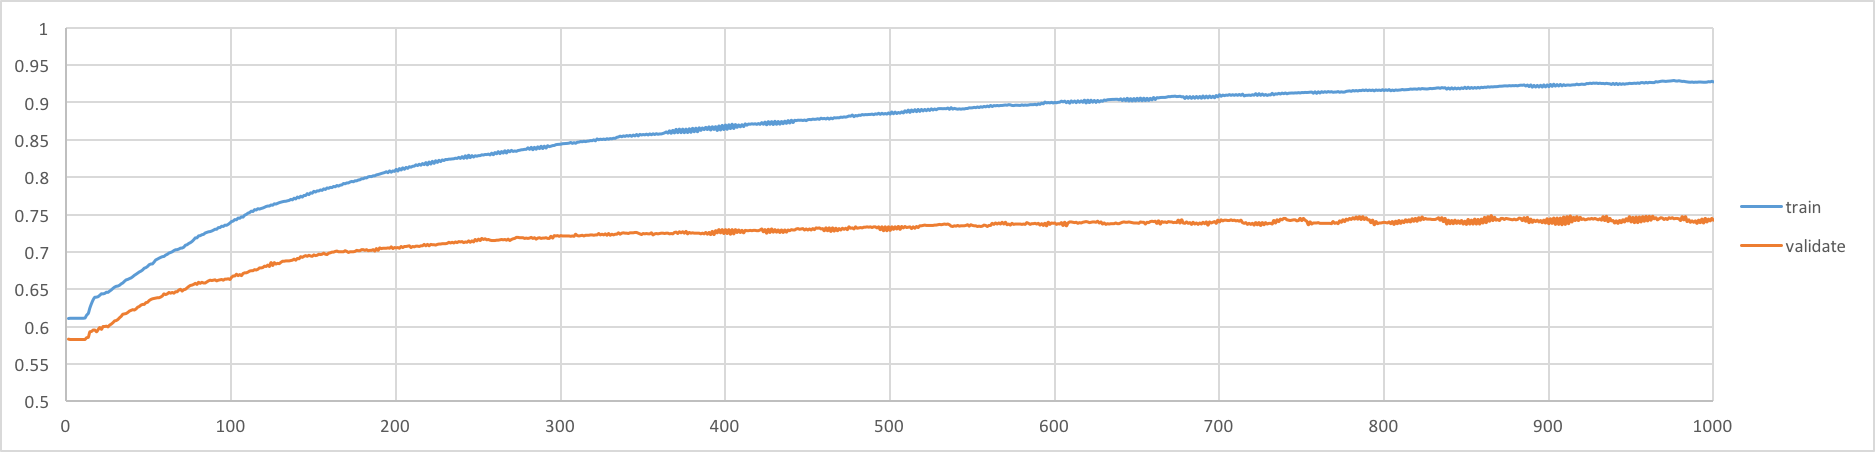
\includegraphics[width=1.0\columnwidth]{I2_uni.png}}\\%
	\subfigure[]{\label{fig:b}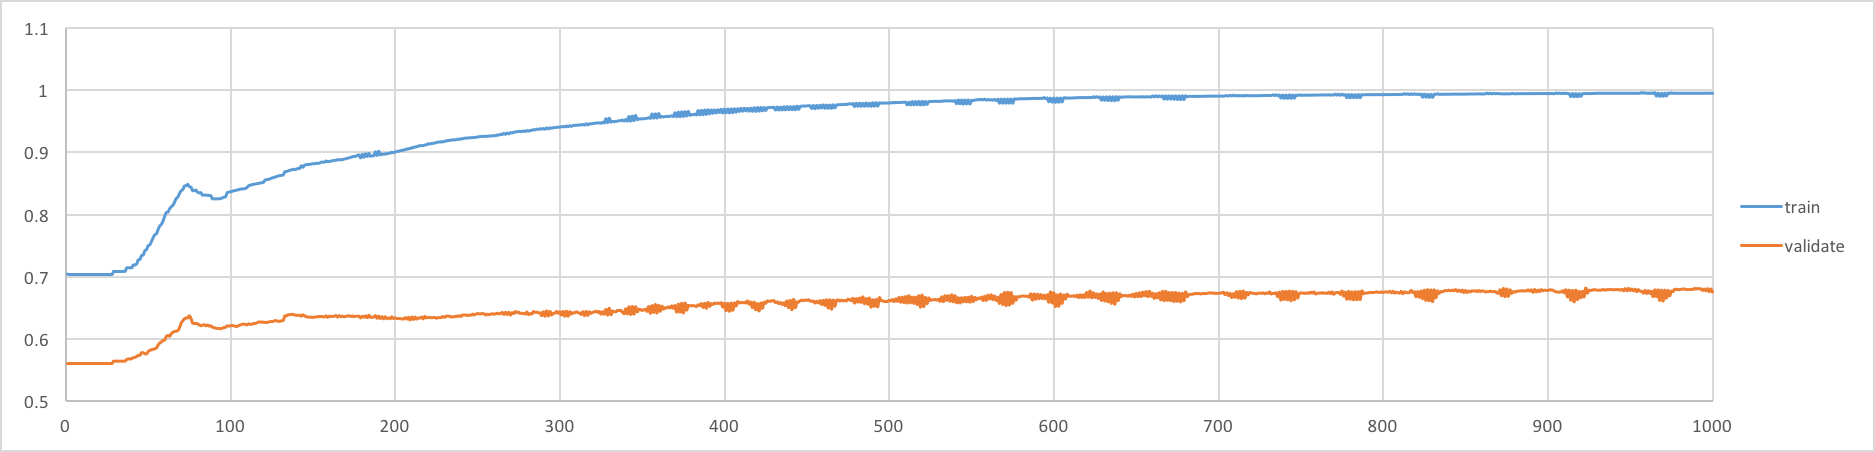
\includegraphics[width=1.0\columnwidth]{I2_bi.png}}\\ % 
	\subfigure[]{\label{fig:c} 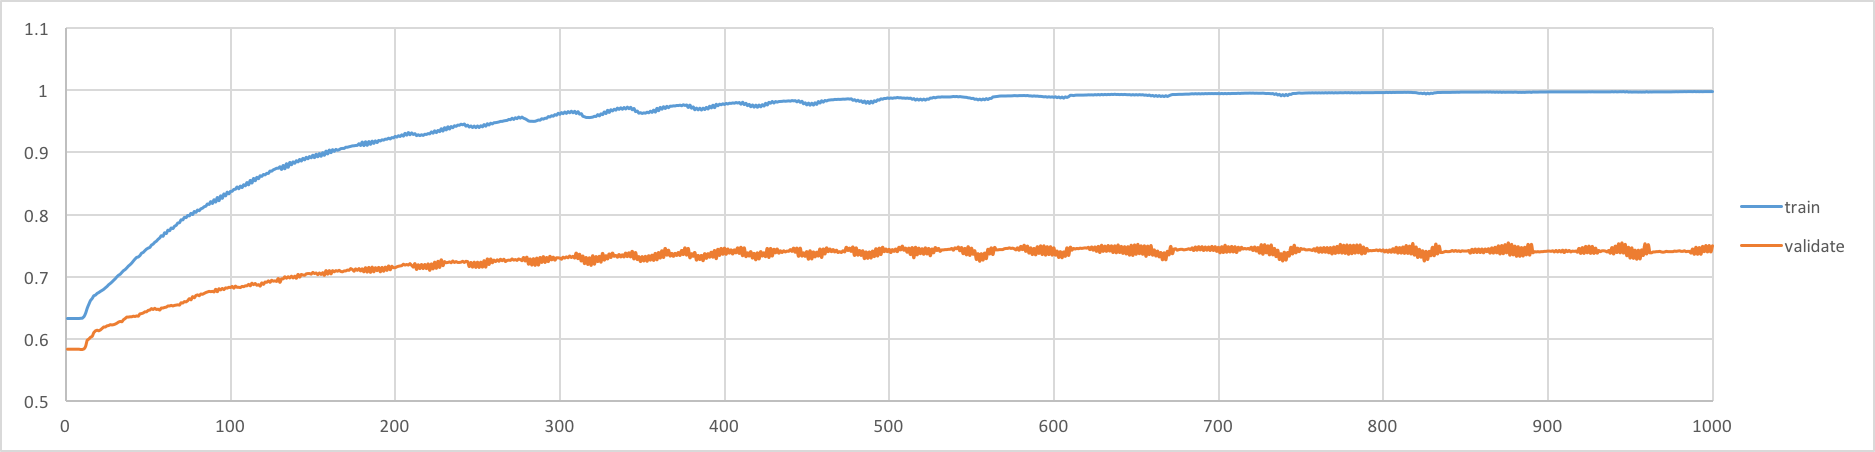
\includegraphics[width=1.0\columnwidth]{I2_both.png}}% 
%  \subfigure[Fibers bonded in the network.]{\label{fig:microstructure_mag} \includegraphics[width=0.5\columnwidth]{microstructure_mag.jpg}}% 
  \caption{Accuracy of training and validation set for different feature sets with I2 norm.}
  \label{fig:I2_accuracy}
\end{figure}

\begin{figure}[!h]
  \centering 
	\subfigure[]{\label{fig:a}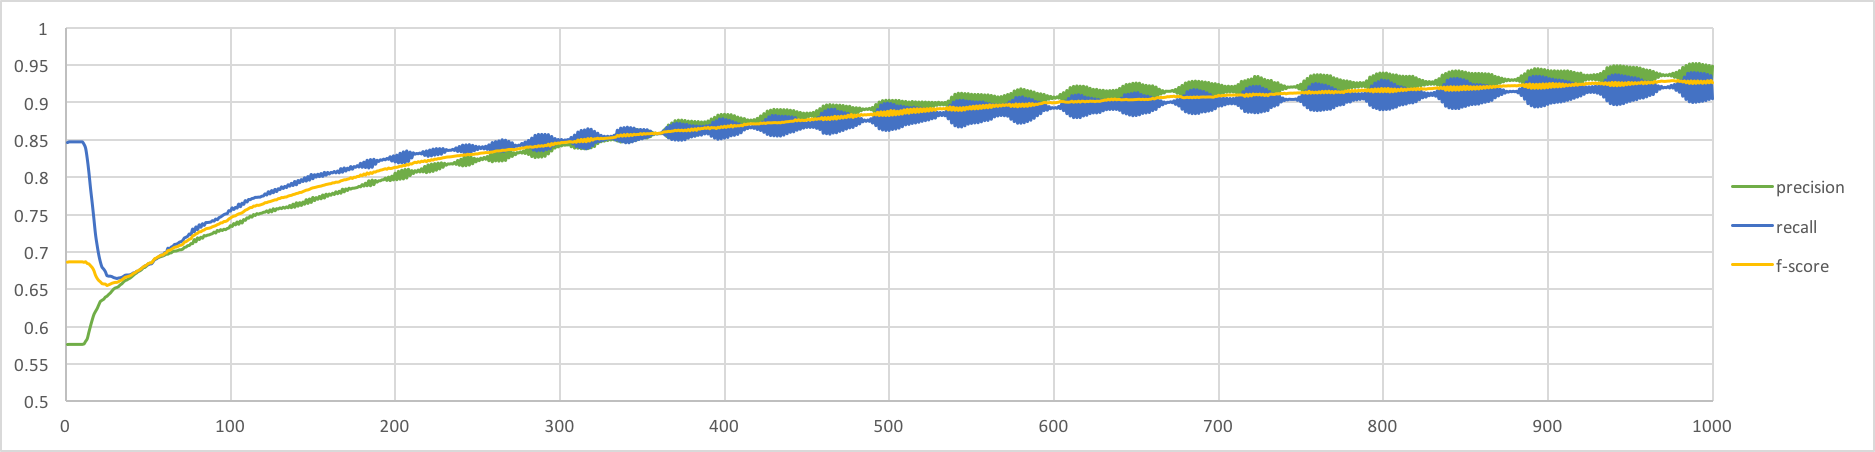
\includegraphics[width=1.0\columnwidth]{I2_uni_tr.png}}\\%
	\subfigure[]{\label{fig:b}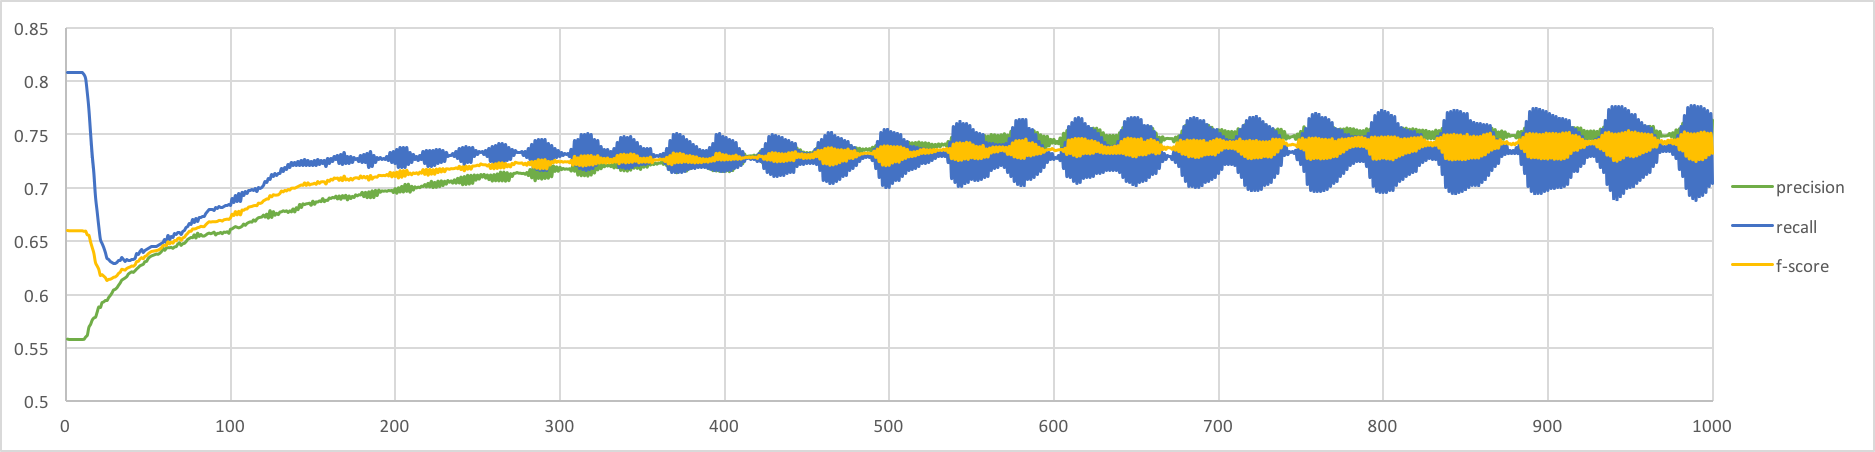
\includegraphics[width=1.0\columnwidth]{I2_uni_va.png}}%  
%  \subfigure[Fibers bonded in the network.]{\label{fig:microstructure_mag} \includegraphics[width=0.5\columnwidth]{microstructure_mag.jpg}}% 
  \caption{Performance of (a) training and (b) validation set for unigram feature sets with I2 norm.}
  \label{fig:I2_unigram}
\end{figure}

\begin{figure}[!h]
  \centering 
	\subfigure[]{\label{fig:a}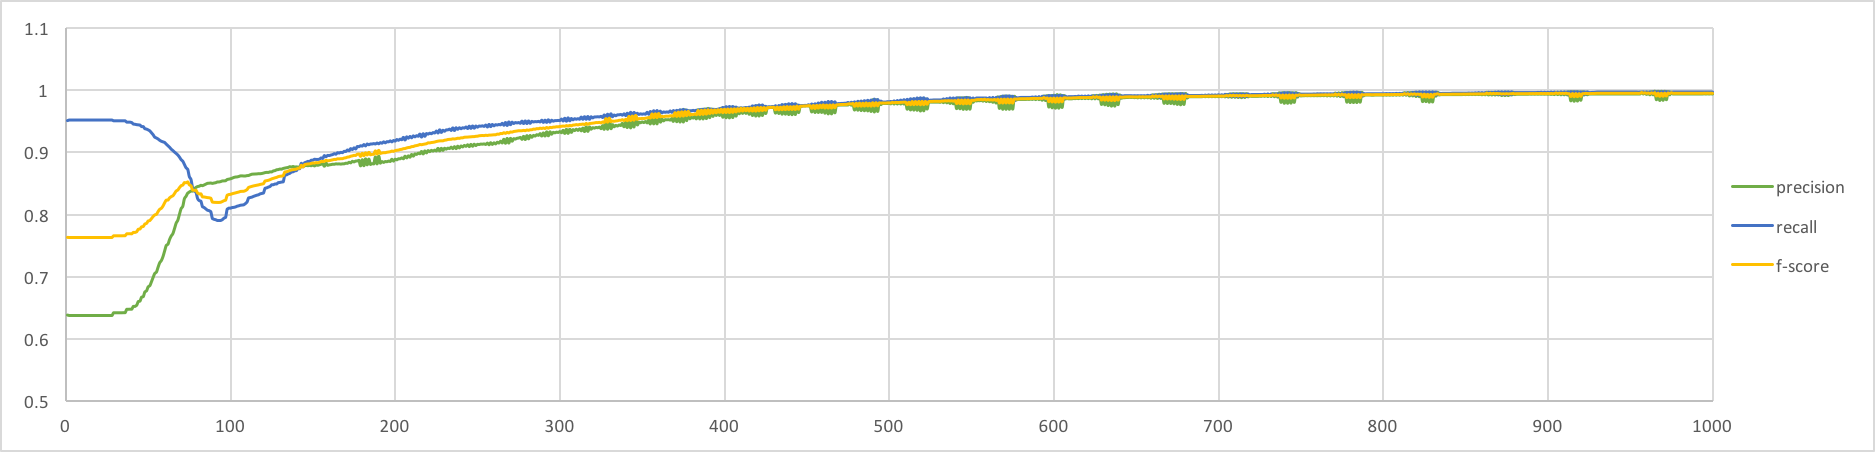
\includegraphics[width=1.0\columnwidth]{I2_bi_tr.png}}\\%
	\subfigure[]{\label{fig:b}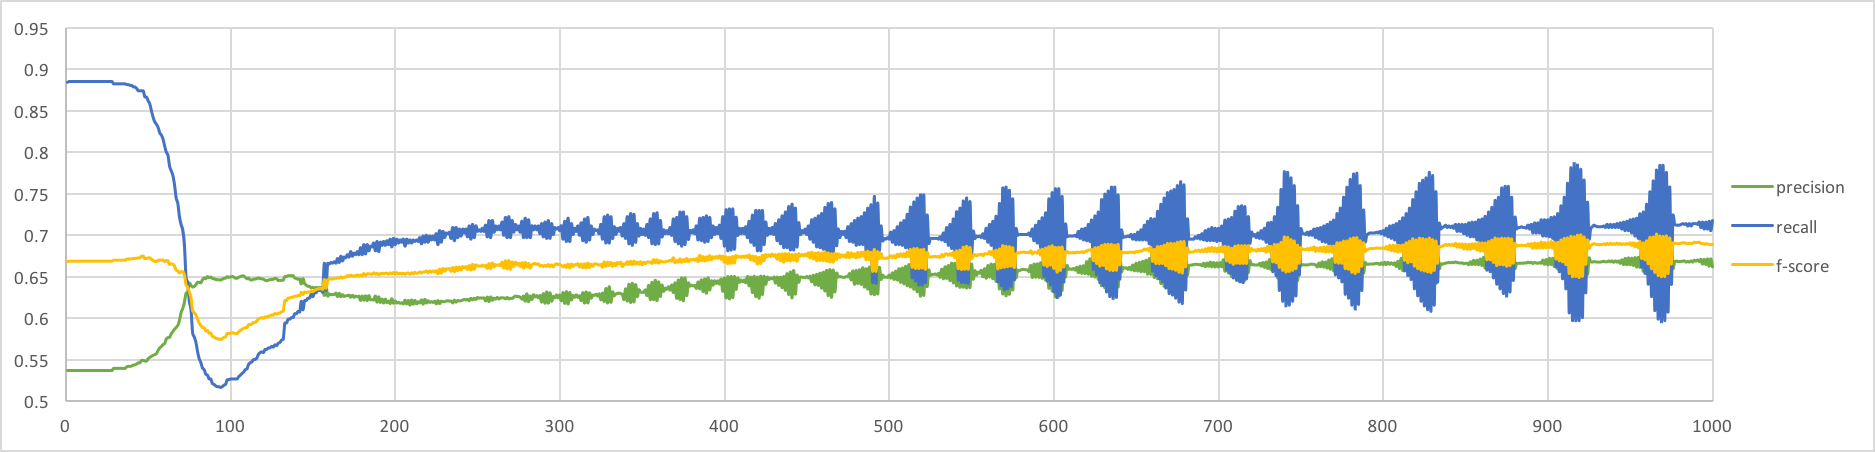
\includegraphics[width=1.0\columnwidth]{I2_bi_va.png}}%  
%  \subfigure[Fibers bonded in the network.]{\label{fig:microstructure_mag} \includegraphics[width=0.5\columnwidth]{microstructure_mag.jpg}}% 
  \caption{Performance of (a) training and (b) validation set for bigram feature sets with I2 norm.}
  \label{fig:I2_bigram}
\end{figure}

\begin{figure}[!h]
  \centering 
	\subfigure[]{\label{fig:a}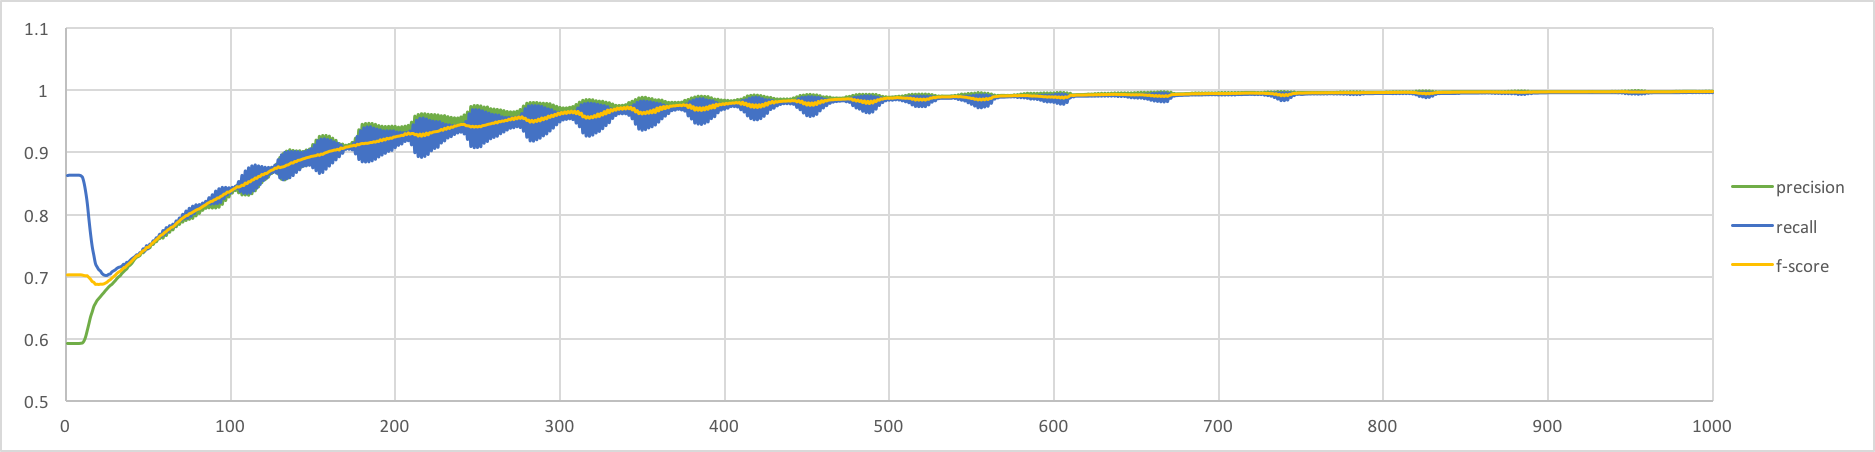
\includegraphics[width=1.0\columnwidth]{I2_both_tr.png}}\\%
	\subfigure[]{\label{fig:b}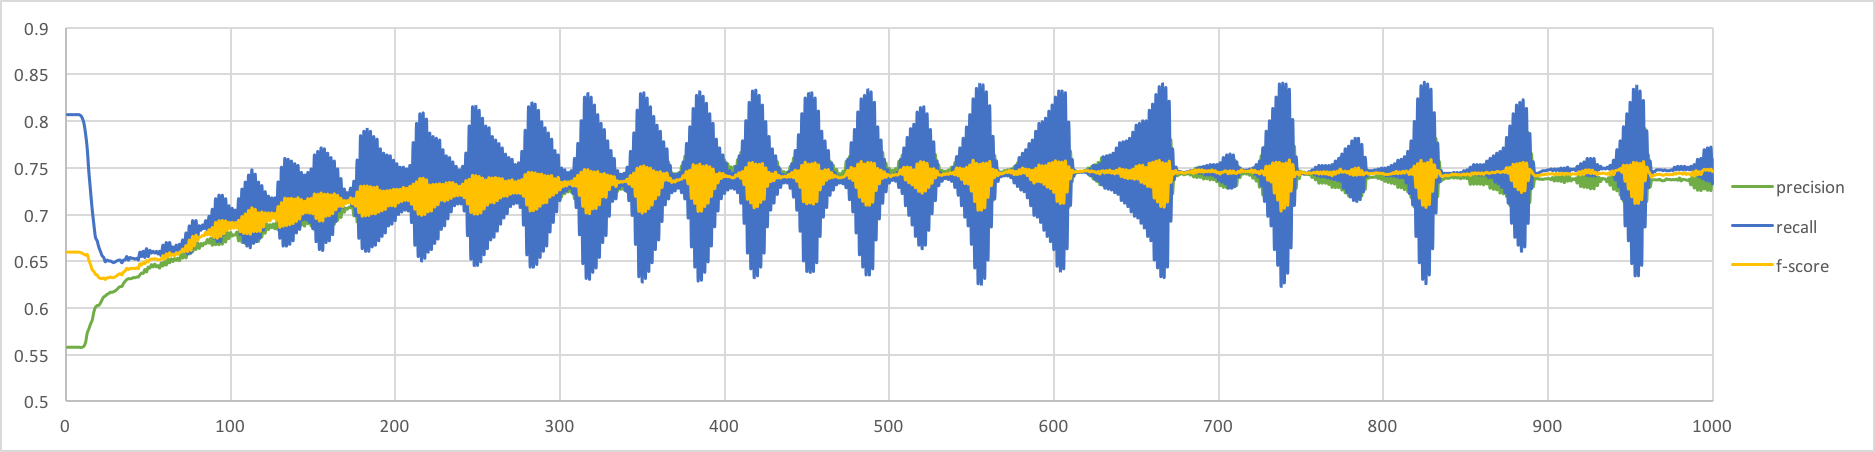
\includegraphics[width=1.0\columnwidth]{I2_both_va.png}}%  
%  \subfigure[Fibers bonded in the network.]{\label{fig:microstructure_mag} \includegraphics[width=0.5\columnwidth]{microstructure_mag.jpg}}% 
  \caption{Performance of (a) training and (b) validation set for both feature sets with I2 norm.}
  \label{fig:I2_bogram}
\end{figure}

%\nocite{*}
%\bibliographystyle{plainnat}
%\bibliography{all}

\end{document}
